% vim: set spell spelllang=en tw=100 :

\documentclass[letterpaper]{article}
\usepackage[pass]{geometry}

\usepackage{ijcai16}
\usepackage{times}
\usepackage{complexity}
\usepackage{microtype}
\usepackage{gnuplot-lua-tikz}
\usepackage{amsmath}
\usepackage{amssymb}
\usepackage{placeins}
\usepackage{cleveref}
\usepackage{natbib}
\usepackage{dblfloatfix}

% \usepackage{showframe}

\usetikzlibrary{decorations, decorations.pathreplacing, calc, backgrounds}

\definecolor{uofguniversityblue}{rgb}{0, 0.219608, 0.396078}

\definecolor{uofgheather}{rgb}{0.356863, 0.32549, 0.490196}
\definecolor{uofgaquamarine}{rgb}{0.603922, 0.72549, 0.678431}
\definecolor{uofgslate}{rgb}{0.309804, 0.34902, 0.380392}
\definecolor{uofgrose}{rgb}{0.823529, 0.470588, 0.709804}
\definecolor{uofgmocha}{rgb}{0.709804, 0.564706, 0.47451}
\definecolor{uofgsandstone}{rgb}{0.321569, 0.278431, 0.231373}
\definecolor{uofgforest}{rgb}{0, 0.2, 0.129412}
\definecolor{uofglawn}{rgb}{0.517647, 0.741176, 0}
\definecolor{uofgcobalt}{rgb}{0, 0.615686, 0.92549}
\definecolor{uofgturquoise}{rgb}{0, 0.709804, 0.819608}
\definecolor{uofgsunshine}{rgb}{1.0, 0.862745, 0.211765}
\definecolor{uofgpumpkin}{rgb}{1.0, 0.72549, 0.282353}
\definecolor{uofgthistle}{rgb}{0.584314, 0.070588, 0.447059}
\definecolor{uofgrust}{rgb}{0.603922, 0.227451, 0.023529}
\definecolor{uofgburgundy}{rgb}{0.490196, 0.133333, 0.223529}
\definecolor{uofgpillarbox}{rgb}{0.701961, 0.047059, 0}
\definecolor{uofglavendar}{rgb}{0.356863, 0.301961, 0.580392}

\renewcommand{\topfraction}{0.9}
\renewcommand{\bottomfraction}{0.8}
\renewcommand{\dbltopfraction}{0.9}
\renewcommand{\textfraction}{0.05}
\setcounter{dbltopnumber}{2}
\renewcommand{\floatpagefraction}{0.85}
\renewcommand{\dblfloatpagefraction}{0.85}

% cref style
\crefname{figure}{Figure}{Figures}
\Crefname{figure}{Figure}{Figures}

% http://tex.stackexchange.com/questions/22100/the-bar-and-overline-commands
\newcommand{\shortoverline}[1]{\mkern 1.5mu\overline{\mkern-1.5mu#1\mkern-1.5mu}\mkern 1.5mu}

\title{Heuristics and Really Hard Instances for Subgraph Isomorphism Problems}
\author{Ciaran McCreesh\thanks{This work was supported by the Engineering and Physical Sciences
    Research Council [grant number EP/K503058/1]} \and Patrick Prosser \and James Trimble \\
University of Glasgow, Glasgow, Scotland \\
c.mccreesh.1@research.gla.ac.uk}

\begin{document}

\maketitle

\begin{abstract}
    We show how to generate ``really hard'' random instances for variants of the subgraph
    isomorphism problem. For the non-induced variant, we predict and observe a phase
    transition between satisfiable and unsatisfiable instances, with a corresponding complexity peak
    in three different solvers. For the induced variant, much richer behaviour is observed, and we
    see evidence that constrainedness is a better measure of difficulty than proximity to a phase
    transition. Finally, we show that existing heuristics for the non-induced variant can be
    recovered by determining how to maximise the expected number of solutions, and that this
    technique gives new, better heuristics for the induced variant.
\end{abstract}

\section{Introduction}

The \emph{non-induced subgraph isomorphism problem} is to find an injective mapping from a given
pattern graph to a given target graph which preserves adjacency---in essence, we are ``finding a
copy of'' the pattern inside the target. The \emph{induced} variant of the problem additionally
requires that the mapping preserve non-adjacency, so there are no ``extra edges'' in the copy of the
pattern that we find. We illustrate both variants in \cref{figure:sip}.
Despite these problems being \NP-complete, modern practical subgraph isomorphism algorithms can
handle problem instances with many hundreds of vertices in the pattern graph, and up to ten thousand
vertices in the target graph \citep{Cordella:2004,Solnon:2010,Audemard:2014,McCreesh:2015}, leading
to successful application in areas such as computer
vision \citep{Damiand:2011,Solnon:2015}, biochemistry \citep{Giugno:2013}, and pattern recognition
\citep{Conte:2004}.

\begin{figure}[b]
    \centering
    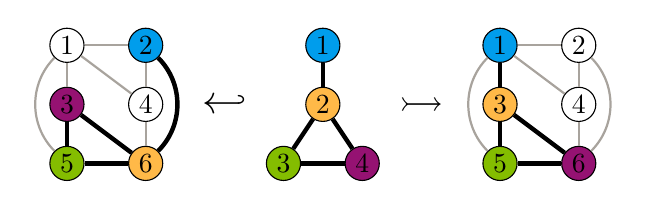
\begin{tikzpicture}[scale=0.5]
        \begin{scope}
            \node [draw, circle, fill=uofgcobalt, inner sep=1.5pt] (Na) at (1,  0) {1};
            \node [draw, circle, fill=uofgpumpkin, inner sep=1.5pt] (Nb) at (1, -1.5) {2};
            \node [draw, circle, fill=uofglawn, inner sep=1.5pt] (Nc) at (0, -3) {3};
            \node [draw, circle, fill=uofgthistle, inner sep=1.5pt] (Nd) at (2, -3) {4};

            \draw [ultra thick] (Na) -- (Nb);
            \draw [ultra thick] (Nb) -- (Nc);
            \draw [ultra thick] (Nc) -- (Nd);
            \draw [ultra thick] (Nb) -- (Nd);

            \node [draw, circle, fill=uofgcobalt, inner sep=1.5pt] (N1) at (5.5,  0) {1};
            \node [draw, circle, fill=white, inner sep=1.5pt] (N2) at (7.5,  0) {2};
            \node [draw, circle, fill=uofgpumpkin, inner sep=1.5pt] (N3) at (5.5, -1.5) {3};
            \node [draw, circle, fill=white, inner sep=1.5pt] (N4) at (7.5, -1.5) {4};
            \node [draw, circle, fill=uofglawn, inner sep=1.5pt] (N5) at (5.5, -3) {5};
            \node [draw, circle, fill=uofgthistle, inner sep=1.5pt] (N6) at (7.5, -3) {6};

            \draw [thick, color=uofgsandstone!50] (N1) -- (N2);
            \draw [ultra thick] (N1) -- (N3);
            \draw [thick, color=uofgsandstone!50] (N1) -- (N4);
            \draw [thick, color=uofgsandstone!50] (N2) -- (N4);
            \draw [ultra thick] (N3) -- (N5);
            \draw [ultra thick] (N3) -- (N6);
            \draw [thick, color=uofgsandstone!50] (N4) -- (N6);
            \draw [ultra thick] (N5) -- (N6);
            \draw [thick, color=uofgsandstone!50] (N2) to [in=45, out=315] (N6);
            \draw [thick, color=uofgsandstone!50] (N1) to [in=135, out=225] (N5);

            \node [draw, circle, fill=white, inner sep=1.5pt] (M1) at (-5.5,  0) {1};
            \node [draw, circle, fill=uofgcobalt, inner sep=1.5pt] (M2) at (-3.5,  0) {2};
            \node [draw, circle, fill=uofgthistle, inner sep=1.5pt] (M3) at (-5.5, -1.5) {3};
            \node [draw, circle, fill=white, inner sep=1.5pt] (M4) at (-3.5, -1.5) {4};
            \node [draw, circle, fill=uofglawn, inner sep=1.5pt] (M5) at (-5.5, -3) {5};
            \node [draw, circle, fill=uofgpumpkin, inner sep=1.5pt] (M6) at (-3.5, -3) {6};

            \draw [thick, color=uofgsandstone!50] (M1) -- (M2);
            \draw [thick, color=uofgsandstone!50] (M1) -- (M3);
            \draw [thick, color=uofgsandstone!50] (M1) -- (M4);
            \draw [thick, color=uofgsandstone!50] (M2) -- (M4);
            \draw [ultra thick] (M3) -- (M5);
            \draw [ultra thick] (M3) -- (M6);
            \draw [thick, color=uofgsandstone!50] (M4) -- (M6);
            \draw [ultra thick] (M5) -- (M6);
            \draw [ultra thick] (M2) to [in=45, out=315] (M6);
            \draw [thick, color=uofgsandstone!50] (M1) to [in=135, out=225] (M5);

            \node [anchor=center, font=\Large] (A1) at (-1.5, -1.5) { $\hookleftarrow$ };
            \node [anchor=center, font=\Large] (A2) at ( 3.5, -1.5) { $\rightarrowtail$ };
        \end{scope}
    \end{tikzpicture}

    \caption{There is a non-induced isomorphism from the pattern graph, in the center, to the target
    on the right, mapping vertex 1 to 1, 2 to 3, 3 to 5 and 4 to 6. This is not an induced
    isomorphism, since there is an edge between 1 and 5 in the target but not between 1 and 3 in the
    pattern. The mapping from the pattern to the (same) target on the left, sending 1 to 2, 2 to 6,
    3 to 5 and 4 to 3, is both non-induced and induced.}
    \label{figure:sip}
\end{figure}

However, these algorithms cannot handle \emph{arbitrary} instances of this size. The experimental
evaluations of these algorithms were performed using a mix of real-world graphs, graphs that encode
biochemistry and computer vision problems, and randomly generated graph pairs. Using random
instances to evaluate algorithm behaviour can be beneficial, because it provides a way of generating
many instances cheaply, and reduces the risk of over-fitting when tuning design parameters. The
random instances used in each case came from common datasets \citep{DeSanto:2003,Zampelli:2010},
which were generated by taking a random subgraph of a random graph (using various models, including
Erd\H{o}s-R\'enyi, scale-free, bounded degree, and meshes) and permuting the vertices. Such
instances are guaranteed to be satisfiable---\citet{Anton:2009} exploited this property to create
large sets of random satisfiable SAT instances.  However, since this has been the only approach used
to generate random subgraph isomorphism instances, existing benchmark suites contain relatively few
non-trivial unsatisfiable instances, and the satisfiable instances tend to be computationally fairly
easy, with most of the difficulty being in dealing with the size of the model.  This problem cannot
be addressed by using a pattern graph from one of the random suites with the ``wrong'' target graph:
this tends to give either a trivially unsatisfiable instance, or a satisfiable instance. (In
particular, it is \emph{not} the case that a relatively small random graph is unlikely to appear in
a larger random graph.)

Here we present and evaluate a new method for creating random pattern/target pairs. This method
generates both satisfiable and unsatisfiable instances, and can produce computationally challenging
instances with only a few tens of vertices in the pattern, and 150 vertices in the target. Our work
builds upon the phase transition phenomena observed in satisfiability and graph colouring problems
first described by \citet{Cheeseman:1991} and \citet{Mitchell:1992}---?? cite later stuff and
explain really hard.

For subgraph isomorphism we identify relevant control parameters: we can independently alter the
edge probability of the pattern graph, the edge probability of the target graph, and the relative
orders (number of vertices) of the pattern and target graphs.  For non-induced isomorphisms, with
the correct choice of parameters we see results very similar to those observed with boolean
satisfiability problems: there is a phase transition from satisfiable to unsatisfiable (and we can
predict its location), and we see a complexity peak occur with three different solvers near this
phase transition.

For certain choices of parameters for induced isomorphisms, there are two phase transitions, going
from satisfiable to unsatisfiable, and then from unsatisfiable back to satisfiable. Again, when
going from satisfiable to unsatisfiable (from either direction), instances go from being trivial to
really hard to solve. However, each of the three solvers we tested also finds the central
unsatisfiable region to be really hard---this may be unexpected, since this region is not near a
phase transition. To show that this is not a simple weakness of current subgraph isomorphism
algorithms, we verify that this region is also hard when using use a pseudo-boolean encoding, and
under reduction to the clique problem. Interestingly, the constrainedness measure
\citep{Gent:1996:Kappa} \emph{does} predict this difficult region---these instances provide (?? the
first??) evidence in favour of constrainedness, rather than proximity to a phase transition, being
an accurate predictor of difficulty.

?? Finally, we discuss the relationship between heuristics and the expected number of solutions,
recovering existing heuristics for the non-induced variant, and introducing new heuristics for the
induced variant. I have failed miserably at integrating this paragraph smoothly.

\subsection{Definitions}

Throughout, our graphs are unlabelled, undirected, and do not have any loops (vertices which are
adjacent to themselves).  The \emph{order} of a graph is the cardinality of its vertex set. We write
$\operatorname{V}(G)$ for the vertex set of a graph $G$. The \emph{complement} of a graph $G$,
denoted $\shortoverline{G}$, is the
graph with the same vertex set as $G$, and with an edge between distinct vertices $v$ and $w$ iff
$v$ and $w$ are not adjacent in $G$. We write $G(v, p)$ for an Erd\H{o}s-R\'enyi random graph with
$v$ vertices, and an edge between each distinct pair of vertices with independent probability $p$.

A \emph{non-induced subgraph isomorphism} from a graph $P$ (called the \emph{pattern}) to a graph
$T$ (called the \emph{target}) is an injective mapping from $\operatorname{V}(P)$ to
$\operatorname{V}(T)$ which preserves adjacency---that is, for every adjacent $v$ and $w$ in
$\operatorname{V}(P)$, the vertices $i(v)$ and $i(w)$ are adjacent in $T$. An \emph{induced subgraph
isomorphism} additionally preserves non-adjacency---that is, if $v$ and $w$ are not adjacent in $P$,
then $i(v)$ and $i(w)$ must not be adjacent in $T$. We use the notation $i : P \rightarrowtail T$
for a non-induced isomorphism, and $i : P \hookrightarrow T$ for an induced isomorphism. Observe
that an induced isomorphism $i : P \hookrightarrow T$ is a non-induced isomorphism $i : P
\rightarrowtail T$ which is also a non-induced isomorphism $\shortoverline{i} : \shortoverline{P}
\rightarrowtail \shortoverline{T}$.

\subsection{Experimental Setup}

Our experiments were performed on systems with Intel Xeon E5-4650 v2 (Q1'14) CPUs and 768GBytes RAM
(although this much RAM was not needed), running Scientific Linux release 6.7.   ?? Software
versions: Clasp 3.1.3, Gurobi 6.0.5, Glasgow, LAD version 2, VFLib. Software was compiled using GCC
4.9.

?? Stuff about runtimes and recursive calls. We are not aiming to compare solvers; rather, we are
looking for solver-independent behaviour. We need a quick note on the models used here too.

?? Timeouts

\section{Non-Induced Subgraph Isomorphisms}

\begin{figure}[tb]
    \setlength{\abovecaptionskip}{6pt}
    \input{gen-graph-phase-transition.tex}
    \caption{With a fixed a pattern graph order of 20, a target graph order of 150, a target edge
        probability of 0.4, and varying pattern edge probability, we observe a phase transition and
        complexity peak with the Glasgow solver in the non-induced variant. Each point represents
        one instance. The lines show mean search effort, and mean proportion satisfiable.}
    \label{figure:phase-transition}
\end{figure}

Suppose we arbitrarily decide upon a pattern graph order of 20, a target graph order of 150, and a
fixed target edge probability of 0.40. As we vary the pattern edge probability from 0 to 1, we would
expect to see a shift from entirely satisfiable instances (with no edges in the pattern, we can
always find a match) to entirely unsatisfiable instances (a maximum clique in this order and edge
probability of target graph will usually have between 9 and 12 vertices). Indeed,
\cref{figure:phase-transition} shows that this is the case: the line (and the points show a subset
of the samples) ?? describe this a bit more, find the 0.5 SAT mark.

?? Some stuff about the complexity peak in the Glasgow solver. This looks remarkably similar to random
3SAT problems---compare, for example, Figure 1 of \citet{LeytonBrown:2014}. In particular,
satisfiable instances tend to be easier but show greater variation than unsatisfiable instances, and
there are exceptionally hard satisfiable instances \citep{Smith:1997}.

?? Are unsatisfiable instances on the phase transition much harder than satisfiable ones?

\begin{figure}[tb]
    \setlength{\abovecaptionskip}{0pt}
    \input{gen-graph-non-induced.tex}
    \caption{Behaviour of algorithms on the non-induced variant. For each plot, the x-axis is the
        pattern edge probability and the y-axis is the target edge probability, both from 0 to 1.
        Along the top row, we show the proportion of instances which are satisfiable; the white
        bands shows the phase transitions, and the black lines are our predictions of where the
        phase transition will occur. On the second row, we show the number of search nodes used by the
        Glasgow algorithm, on the third row, the number of search nodes used by the LAD algorithm, and the
        fourth, VF2; the dark regions indicate ``really hard'' instances.}
    \label{figure:non-induced}
\end{figure}

What if we alter the edge probabilities for both the pattern graph and the target graph?  In the top
row of \cref{figure:non-induced} we show the phase transition for the non-induced variant, for
patterns of order 10, 20 and 30, a target of order 150, and varying pattern (x-axis) and target
(y-axis) edge probabilities. Each axis runs over 51 edge probabilities, from 0 to 1 in steps of
0.05; for each of these 2601 points, we generate ten random instances. The colour denotes (?? wrong
word?) the proportion of these instances which were found to be satisfiable.  Inside the orange
region, at the bottom right of each plot, every instance is unsatisfiable---here we are trying to
find a dense pattern in a sparse target. In the purple region, at the top left, every instance is
satisfiable---we are looking for a sparse pattern in a dense target (which is easy, since we only
have to preserve adjacency, not non-adjacency). The white band between the regions shows the
location of the phase transition: here, roughly half the instances are satisfiable. (We discuss the
black line below.)

On subsequent rows, we show the average number of search nodes used by the different algorithms. In
general, satisfiable instances are easy, until very close to the phase transition. As we hit the
phase transition and move into the unsatisfiable region, we see a complexity increase. Finally, as
we pass the phase transition and move deeper into the unsatisfiable region, instances become easier
again. This behaviour is largely solver-independent, although VF2 has a larger hard region than
Glasgow or LAD. Thus, although we have moved away from the single control parameter typically
studied, we observe similar behaviour to other \NP-complete problems.

\subsection{Locating the Phase Transition}

To predict the location of the phase transition, we can calculate the expected number of solutions
by making a few dubious assumptions involving rounding and independence. Since we are trying to find
an \emph{injective} mapping from a pattern $P = G(p, d_p)$ to a target $T = G(t, d_t)$, there are
$t^{\underline{p}} = t \cdot (t - 1) \cdot \ldots \cdot (t - p + 1)$ possible assignments of target
vertices to pattern vertices.  We expect the pattern to have $d_p \cdot \binom{p}{2}$ edges, so we
obtain the probability of all of these edges being mapped to edges in the target by raising $d_t$ to
this power, giving an expected number of solutions of \[ \langle Sol \rangle = t^{\underline{p}}
\cdot {d_t}^{d_p \cdot \binom{p}{2}} \textnormal{.} \] This formula predicts a very sharp phase
transition from $\langle Sol \rangle \ll 1$ to $\langle Sol \rangle \gg 1$. We plot where this
occurs using black lines in the first row of \cref{figure:non-induced}.

We can see that this prediction is generally accurate, except that for very low and very high
pattern densities, we overestimate the satisfiable region slightly. This is because although an
expected number of solutions much below one implies a high likelihood of unsatisfiability, it is not
true that a high expected number of solutions implies that any particular instance is likely to be
satisfiable---a similar behaviour is seen with random constraint satisfaction problems
\citep{Smith:1994,Smith:1996}.

?? Also because of half edges.

?? Note that the size of the state space is defined differently to in binary CSPs: we're using the
all diff constraint to determine the size of the state space, and are not treating it as a
constraint. In other words, our generate-and-test approach is alldiff-aware. This matters for kappa.

\subsection{Variable and Value Ordering Heuristics}

When designing variable and value ordering heuristics for backtracking search algorithms, there are
various general principles which appear to be effective---one of these is to try to maximise the
expected number of solutions inside any subproblem considered during search \citep{Gent:1996:EN}.
This is usually done by cheaper surrogates, rather than direct calculation. When branching, both LAD
and Glasgow will pick a variable with fewest remaining values in its domain: doing this will
generally reduce the first part of the $\langle Sol \rangle$ equation by as little as possible. When
two or domains are of equal size, LAD simply breaks ties lexicographically. Glasgow, however, will
pick a variable corresponding to a pattern vertex of highest degree. This strategy was determined
empirically, but could have been derived from the $\langle Sol \rangle$ formula: picking a
pattern vertex of high degree will make the remaining pattern subgraph sparser, which will decrease
the exponent in the second half of the formula, maximising the overall value. LAD does not apply a
value ordering heuristic, but Glasgow does: it prefers target vertices of lowest degree. Again, this
was determined empirically, but it has the effect of increasing $\langle Sol \rangle$ by increasing
the remaining target density.

The VF2 heuristics, in contrast, are based around preserving connectivity. This perhaps explains
some of VF2's weakness on graphs that are not extremely sparse.

\section{Induced Isomorphisms}

\begin{figure*}[p]
    \input{gen-graph-induced.tex}
    \caption{Behaviour of algorithms on the induced variant, shown in the style
    of \cref{figure:non-induced}. The second, third and fourth rows show the number of search nodes used by the
    Glasgow, LAD and VF2 algorithms. The fifth row shows a bound on the satisfiable region, by
    considering where a \emph{non-}induced isomorphism may also be a non-induced isomorphism between
    complement graphs. The sixth row plots constrainedness: the darkest region is where
    constrainedness is exactly one, and the lighter regions show where the problem is either over-
    or under-constrained. The final row shows when the Glasgow algorithm performs better when given
    the complements of the pattern and target graphs as
inputs.}\label{figure:induced}
\end{figure*}

In \cref{figure:induced} we repeat our experiments, finding induced isomorphisms. With a pattern of
order 10, we get two independent phase transitions (?? describe properly). For each of the solvers,
the satisfiable instances before either phase transition are generally easy, instances near the
phase transition are hard, and the large central unsatisfiable region is again easy.

?? For larger patterns of order 20 and 30, we have large unsatisfiable regions in the middle,
but these remain hard.

Pattern orders 14, 15 and 16 show the transition between the two styles.

\subsection{Predicting Induced Behaviour}

By repeating the argument for locating the non-induced phase transition and additionally considering
non-edges, we get an expected number of solutions of \[ \langle Sol \rangle = t^{\underline{p}}
    \cdot {d_t}^{d_p \cdot \binom{p}{2}} \cdot {(1 - d_{t})}^{(1 - d_{p}) \cdot \binom{p}{2}}
\textnormal{.} \] We plot this
using black lines on \cref{figure:induced}---again, our prediction is accurate except for very
sparse or very dense patterns.

\subsection{Why is the Central Region Hard?}

?? Explain the flip bound on row 5, and note that the difficult region is roughly near the phase
transitions in the original graphs.

?? Note that the large unexpectedly hard region in the middle is solver-independent. Perhaps
subgraph isomorphism algorithms are not able to make use of adjacency and non-adjacency
simultaneously, and this is a weakness in how all three are designed? In the following section we
debunk this wonderful hypothesis.

?? Constrainedness predicts the hard region in the middle \citep{Gent:1996:Kappa}! Add a two line
description of kappa, the slightly modified way we calculated it. We plot this on the sixth row of
\cref{figure:induced}.

?? Maybe note a few solver-dependent hard instances.  There's odd unsat with LAD at the top right
(not EHPs), trivial for Glasgow: mapping a non-clique into a clique. Glasgow looks at non-edges and
can see immediately that no mapping is possible, but LAD doesn't do degree filtering on complements.

\subsection{New Heuristics}

?? Explain why we might guess degree heuristics just won't work for induced: for everything we say
about degree, the opposite holds too for the complement constraints.

?? Explain bottom row of \cref{figure:induced}, and give way of calculating it. The key point is
that depending upon where we are, changes to one of the two terms has more effect in the equation.
Note how sharp and well-defined this is.

?? Possibly send the data to Lars, and get him to run his portfolios stuff on it, and then make fun
of machine learning?

?? Note that when the pattern is small, it is always best to try to move towards the satisfiable
region, even for unsatisfiable instances. It's not clear what's going on when the pattern is large.
Note the suggestion by \citet{Walsh:1998} that switching heuristics based upon an estimate of the
solubility of the problem may offer good performance.

?? Is this heuristic better in general, on non-random instances? Unfortunately most of the instances
in the standard benchmark set are too sparse for it to kick in. However, it provides a justification
for reusing the non-induced heuristics.

\section{Other Encodings and Solvers}

\begin{figure*}[t]
    \setlength{\abovecaptionskip}{0pt}
    \input{gen-graph-sat.tex}
    \caption{Behaviour of other solvers on the induced variant on smaller graphs, shown in the style of
        \cref{figure:non-induced}. The second row shows the number of search nodes used by the
    Glasgow algorithm, the third row shows the number of decisions made by the Clasp pseudo-boolean
solver, and the fourth row shows the number of search nodes used by BBMC on the clique
encoding.}\label{figure:alt}
\end{figure*}

The region in the parameter space where both pattern and target have medium density is far from a
phase transition, but nevertheless contains instances that are hard for current subgraph isomorphism
solvers. We would like to know whether this is due to a weakness in current solvers, or whether
instances in this region are inherently difficult to solve, as constrainedness suggests. In
\cref{figure:alt} we repeat the induced experiments on smaller pattern and target graphs, using
different solving techniques.  Although these techniques are not competitive in absolute terms, we
wish to see if the same pattern of behaviour occurs.

We create a pseudo-boolean (PB) encoding as follows. For each pattern vertex $v$ and each target
vertex $w$, we have a binary variable which takes the value 1 if and only if that $v$ is mapped to
$w$.  Constraints are added to ensure that each pattern vertex maps to exactly one target vertex,
that each target vertex is mapped to by at most one pattern vertex, that adjacent vertices are
mapped to adjacent vertices, and that non-adjacent vertices are mapped to non-adjacent vertices. We
used the Clasp solver~\citep{gekakaosscsc11a} to solve the pseudo-boolean instances. The instances
that are hard for the Glasgow solver remain hard for the PB solver, including instances inside the
central region, and the easy satisfiable instances remain easy.

We implemented an equivalent SAT encoding with direct encoding of the cardinality constraints. Using
the Glucose solver, we saw very similar performance to the PB encoding. We also implemented a
similar integer program encoding; the Gurobi solver was only able to solve some of the trivial
satisfiable instances, and was almost never able to prove unsatisfiability within the time limit. We
do not plot the results for either of these solvers.

The \emph{association graph encoding} of a subgraph isomorphism problem is constructed by creating a
new graph with a vertex for each pair $(p, t)$ of vertices from the pattern and target graphs
respectively. There is an edge between vertex $(p_1, t_1)$ and vertex $(p_2, t_2)$ if mapping $p_1$
to $t_1$ and $p_2$ to $t_2$ simultaneously is permitted, i.e.\ $p_1$ is adjacent to $p_2$ if and
only if $t_1$ is adjacent to $t_2$. A clique of size equal to the order of the pattern graph exists
in the association graph if and only if the problem is satisfiable \citep{Levi:1973}.  We used this
encoding with a version of the BBMC clique algorithm \citep{SanSegundo:2011} modified to solve the
decision problem. Again, the instances in the central region remain hard, and additionally, some of
the easy satisfiable instances become hard.

These results suggest that the central region may be genuinely hard, despite not being near a phase
transition, and that constrainedness is the better measure of difficulty. The clique encoding in
particular rules out the hypothesis that subgraph isomorphism solvers only find this region hard due
to not reasoning simultaneously about adjacency and non-adjacency, since the association graph
encoding constraints consider compatibility rather than adjacency and non-adjacency.

?? Lends weight to kappa

\section{Conclusion}

?? We found hard instances, some where we'd expect, some in unexpected places. These unexpected
instances, by and large, remained hard under reductions. We looked at how existing non-induced
heuristics could be recovered from Sol, and how this gives us better heuristics for the induced
variant.

?? Consider dynamic heuristics.

?? Other random models and non-random.

?? Does not give hard instances for graph isomorphism.

?? \citep{Lipets:2009} inexact solutions?

\section*{Acknowledgements}

?? I suppose Craig could be given an inkling of undeserved gratitude if we have space left.

\bibliographystyle{named}
\bibliography{paper}

\end{document}
